\section{Binary Experiments and the Budget Curve}\label{app:sign}
\paragraph{The binomial minimax value.}
For any nonzero $d$ set $M=\|d\|_\infty$. With full profiles a randomized sign with conditional mean $Yd(X)/M$ has population mean $\Delta/M$. For $n$ iid signs $W_i$ with unknown mean $\mu_0$, the estimate $\sqrt n\,\overline W/(1+\sqrt n)$ has variance $(1-\mu_0^2)/(1+\sqrt n)^2$ and squared bias $\mu_0^2/(1+\sqrt n)^2$. For the lower bound fix a profile at which $|d|=M$ and vary the sign label. A $\mathrm{Beta}(\sqrt n/2,\sqrt n/2)$ prior on the success probability of the sign makes this constant-risk rule its posterior mean on the mean-sign scale. The Bayes risk equals the displayed frequentist risk, proving minimaxity. The full-profile value is therefore $M^2/(1+\sqrt n)^2$. The one-feature construction in Proposition~\ref{prop:add} simulates these same signs, and the constant-profile lower bound applies. For $M=0$ return zero.

\subsection{Proof of Theorem~\ref{thm:gap}}\label{app:gap}
If $b<2k$, under uniform $X$ the laws $Y=\pm d_k(X)$ give the same observations on every allowed leaf. The risk is at least one and zero attains it. For $b\ge2k$ we show that $J_\U(d_k)=1/C$ and construct a per-person score $H$ with $\E[H\mid X,Y]=Yd_k(X)$ and $\E[H^2\mid X,Y]=C$ for each design type.

\paragraph{Fixed forms.}
Under the uniform law, projecting a multilinear expansion onto a mask retains exactly its contained Fourier terms. In a block of size four a mask with $j=2,3,4$ coordinates captures at most $1/4,1/2,1$ of the total squared coefficient mass, respectively. The first maximum is achieved by a supported pair and the other two by any mask of the indicated size. A block with fewer than two coordinates captures zero mass. Independence of blocks gives total mass at most $2^{b-4k}$, and choosing a supported pair in every two-coordinate block attains it for any budget allocation assigning between two and four coordinates to every block. For two coordinates sample one of four supported pairs uniformly and return twice its signed product. For three, choose $\{1,2,3\}$ or $\{2,3,4\}$ with equal probability. Return $2f$ when the first form is chosen and $x_2=x_3$, or when the second is chosen and $x_2\ne x_3$; return zero otherwise. For four the score is $f$ itself. The scores have conditional means $f$ and constant second moments $4,2,1$. Multiply independently randomized block scores and $Y$ to obtain the desired $H$.

\paragraph{Branching forms.}
When $b=2k+r$, $0\le r\le k$, evaluate $r$ blocks via branching, using three queries each; use a random signed pair score of magnitude two in every other block. Then $H$ has constant absolute value $2^{k-r}$ and square $C=4^{k-r}$. When $b\ge3k$, evaluate every block. For the lower witness, at any deterministic leaf under uniform $X$, an unqueried coordinate remains uniform independent of the others. Nonzero conditional mean for the product requires that every block has at least two exposed coordinates. At most $r$ blocks have more than two, so $|\E_\U[d_k\mid\ell]|\le2^{-(k-r)}$. Averaging yields the bound on $J$. It is attained by evaluating $r$ blocks exactly and querying one predetermined supported pair in each other block. The absolute conditional mean is then $2^{-(k-r)}$ at every leaf.

\paragraph{Exact program and leading coefficients.}
The witness $\mu=\U,h=d_k$ in \eqref{eq:dual} gives $\Phi_n\ge1/(1+n/C)$. Randomized query procedures can be represented as mixtures over deterministic interviews by drawing all their random coins in advance. Taking their unbiased transcript scores with shrinkage $\gamma=n/(n+C)$ gives $s_g=\gamma d_k$ and a second-moment contribution at most $\gamma^2 C$ at every profile. Thus $\Phi_n\le(1-\gamma)^2+\gamma^2 C/n=C/(n+C)$. The same witness in \eqref{eq:vdual} and the unshrunk scores give $V=C$. Theorem~\ref{thm:finite} yields the nonasymptotic rates. At $b\ge3k$, evaluating $d_k$ yields a sign of mean $\Delta$ and the binomial minimax value above.

\paragraph{Exact binary comparison for branching.}
For $2k\le b\le3k$ put $\lambda=2^{b-3k}$. The branching score $\lambda H$ is a sign with mean $\lambda\Delta$ for every $P$. Conversely consider the subfamily of uniform $X$ with conditional label law $(1+\theta y d_k(x))/2$. Then $\Delta=\theta\in[-1,1]$. At each leaf, conditionally on the history and independent random coins, $p_\theta(z)=p_0(z)(1+\theta s_z)$ with $|s_z|\le\lambda$ and $\sum_zp_0(z)s_z=0$. A sign $w$ of mean $\lambda\theta$ can generate this leaf via the probability kernel $K(z\mid w)=p_0(z)(1+w s_z/\lambda)$. Simulating the leaves successively reproduces the complete protocol. This is an explicit experiment comparison in the sense of \citet{blackwell1953}: on the indicated subfamily an arbitrary interview can be simulated using the scalar sign. Together with the construction for every $P$, it gives exact equality of minimax risks with the binary-mean experiment, even for biased estimators.

\paragraph{Why the population supremum matters.}
A uniform-law calculation can be uninformative even when an update is identifiable. For example, take an extra switch $z\in\{-1,1\}$ and set $\widetilde d=1+\mathbf1\{z=1\}(d_k-1)$. This remains Boolean, has degree $2k+1$, and has uniform mean $1/2$, so even an empty form captures at least $1/4$ of the squared mean signal in the uniform witness $h=\widetilde d$. At the identifiable width $2k+1$, however, a population supported on $z=1$ contains the original hard experiment at that width. An auditor given the switch for free still has branching risk of order $\min\{1,4^{k-1}/n\}$ for $k\ge1$. Optimizing over profile laws and perturbations in \eqref{eq:dual} accounts for this possibility.

\begin{figure}[t]
\centering
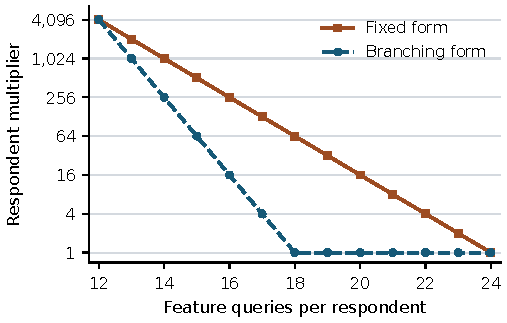
\includegraphics[width=.62\textwidth]{figures/query_cost.pdf}
\caption{Exact synthetic budget curve for the same update on 24 features ($k=6$). The fixed coefficient is 64 and the branching coefficient is one at 18 queries.}
\label{fig:cost}
\end{figure}

